\documentclass[10pt,twocolumn,letterpaper]{article}

\usepackage{cvpr}
\usepackage{times}
\usepackage{epsfig}
\usepackage{graphicx}
\usepackage{amsmath}
\usepackage{amssymb}
\usepackage{booktabs}
\usepackage{multirow}
\usepackage{longtable}

\DeclareMathOperator*{\argmax}{arg\,max}
\DeclareMathOperator*{\argmin}{arg\,min}

\newcommand{\xvec}{\mathbf{x}}
\newcommand{\wvec}{\mathbf{w}}
\newcommand{\R}{\mathbb{R}}

% Include other packages here, before hyperref.

% If you comment hyperref and then uncomment it, you should delete
% egpaper.aux before re-running latex.  (Or just hit 'q' on the first latex
% run, let it finish, and you should be clear).
\usepackage[breaklinks=true,bookmarks=false]{hyperref}

\cvprfinalcopy % *** Uncomment this line for the final submission

\def\cvprPaperID{****} % *** Enter the CVPR Paper ID here
\def\httilde{\mbox{\tt\raisebox{-.5ex}{\symbol{126}}}}

% Pages are numbered in submission mode, and unnumbered in camera-ready
%\ifcvprfinal\pagestyle{empty}\fi
\setcounter{page}{1}
\begin{document}

%%%%%%%%% TITLE
\title{A Highly Versatile Facial Expression Recognition System}

\author{Wei Cui\\
University of Toronto\\
1004536479\\
{\tt\small w.cui@mail.utoronto.ca}
% For a paper whose authors are all at the same institution,
% omit the following lines up until the closing ``}''.
% Additional authors and addresses can be added with ``\and'',
% just like the second author.
% To save space, use either the email address or home page, not both
\and
Kewei Qiu\\
University of Toronto\\
1003798116\\
{\tt\small kewei.qiu@mail.utoronto.ca}
\and
Chenhao Gong\\
University of Toronto\\
1004144598\\
{\tt\small chenhao.gong@mail.utoronto.ca}
}

\maketitle

%%%%%%%%% ABSTRACT
\begin{abstract}
   Facial expression recognition is the operation that analyzes facial expressions on human faces, and connect them to the corresponding emotional states. This report is regarding to a project, conducted by the authors, that suggests a new highly versatile facial expression recognition system, which is based on Fisherfaces algorithm and a Convolutional Neural Network learning model, while supported by the Viola-Jones Feature Detection framework to enable usage in more general scenarios. The report will also compare the system with a number of other popular algorithms and learning models to see how well the system will perform in compasion. 
\end{abstract}

\section{Introduction}
Over the last couple of decades, facial expression analysis has become an overwhelmingly popular topic in computer vision related researches. Facial expressions are the facial changes in response to a person's internal emotions states, intentions, or social communications. Humans can easily tell a person's emotions by looking at their facial expression; whilst, computers need the assistance of a system to analyze the facial expression shown by a human, and connect it to an emotional state known to humans. Such a system is regarded as a facial expression recognition system. 

Prior studies led to the development of a 3-step traditional facial expression analysis thesis, including face localization, feature extraction and expression classification. \cite{Article01} Face localization refers to the step to identify the face in the image so as to enable further analysis on the expressions it is exposing. The Viola-Jones object detection framework is one of the most popular techniques applied in face detection and localization, which features a rapid detection algorithm after the model is trained. \cite{Article02} Feature extration is the step that extracts the significant features that may indicate the facial expression. Either geometric or appearance features shall be extracted for classification. The final step, facial expression classification, is to match the facial expression, demonstrated by the extracted features in the previous step, to the emotions humans are familiar with. In practice, this step is highly related to machine learning, while multiple learning classifier models have been used as found in researches. These include Neural Networks (NN) \cite{Article04}, Support Vector Machines (SVM) \cite{Article05}, Adaboost etc. 

Our highly versatile facial expression recognition system was inspired by and modified from a feature extraction algorithm called ``Fisherfaces'', developed by Peter N. Belhumeur, et al.\cite{Article06} We integrate the algorithm with a convolutional neural network classifier, and implement the Viola-Jones framework \cite{Article02} ahead of it to enable its versatility to operate on any image including a human face. 

\section{Methodology}

\subsection{Viola-Jones Object Detection Framework}
Viola-Jones object detection framework, proposed by Paul Viola and Michael Jones, is a rapid object detection algorithm realized using boosted cascade classifiers. \cite{Article02} This is what we used to detect and align faces from an arbitrary photo.

Viola and Jones' algorithm is a machine learning based algorithm. To train the classifier, a dataset with plenty of positive images (images of faces) and negative images (images without faces) is needed. The first step is to extract features from these images using rectangle-shaped Haar feature filters. Each feature is a single value obtained by subtracting sum of pixels under white rectangle from sum of pixels under black rectangle. Figure ~\ref{fig:haar-feature-filters} provides some examples of Haar feature filters.

To calculate Haar features rapidly, the algorithm uses an intermediate representation for the image called integral image. The integral image at each location $(x, y)$ contains the sum of the pixels above and to the left of $x, y$, inclusive is:
\begin{align*}
ii(x, y) = \sum_{x' \leq x, y' \leq y} i(x', y')
\end{align*}
where $ii(x, y)$ is the integral image and $i(x, y)$ is the original image. Using the following pair of recurrences:
\begin{align*}
    s(x, y) = s(x, y-1) + i(x, y)\\
    ii(x, y) = s(x-1, y) + s(x, y)
\end{align*}
($s(x, y)$ is the cumulative row sum, $s(x, -1) = 0$, and $ii(-1, y) = 0$) the integral image can be computed within one iteration over pixels of the original image. \cite{Article02}

\begin{figure}[t]
\begin{center}
  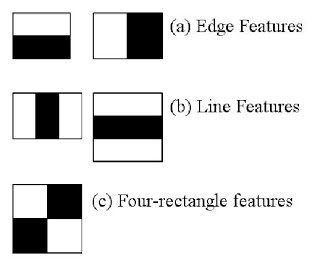
\includegraphics[width=0.8\linewidth]{haar_features.jpg}
  \caption{Example Haar feature filters}
  \label{fig:haar-feature-filters}
\end{center}
\end{figure}

After extract features from images, the alogrithm uses AdaBoost to select the best features out of the large number of extracted feathers. The final classifier is a weighted sum of weak classifiers. According to the paper, even 200 features provide detection with 95\% accuracy. The final classifier has around 6000 features which gives us a precise object detection classifier.

\subsection{Fisherfaces vs. Eigenfaces}
Fisherfaces \cite{Article06} and Eigenfaces \cite{Article07} are two algorithms that were suggested and tested for face recognition, a slightly different problem than what we are interested in.

Over the development of face recognition techniques, Eigenfaces has become one of the popular algorithms with quality outcomes. The essence of the Eigenfaces approach is the use of principal components analysis (PCA) for feature extraction. The algorithm reconstructs a multitude of face images in from the training set by reconstructing them using weighted sums of a small collection of characteristic features (\textit{eigenpictures}), namely \textit{eigenfaces}. After the calculation, it keeps only the images that correspond to the highest eigenvalues in each epoch. \cite{Article07} This is useful to lower the dimensions of the feature space, which is to be fed to the classifier model that follows. However, it yields projection directions that maximize the total scatter across all classes, which contains unwanted variations that are caused by exterior information, i.e. lighting. \cite{Article06}

\begin{figure}[t]
\begin{center}
%\fbox{\rule{0pt}{2in} \rule{0.9\linewidth}{0pt}}
   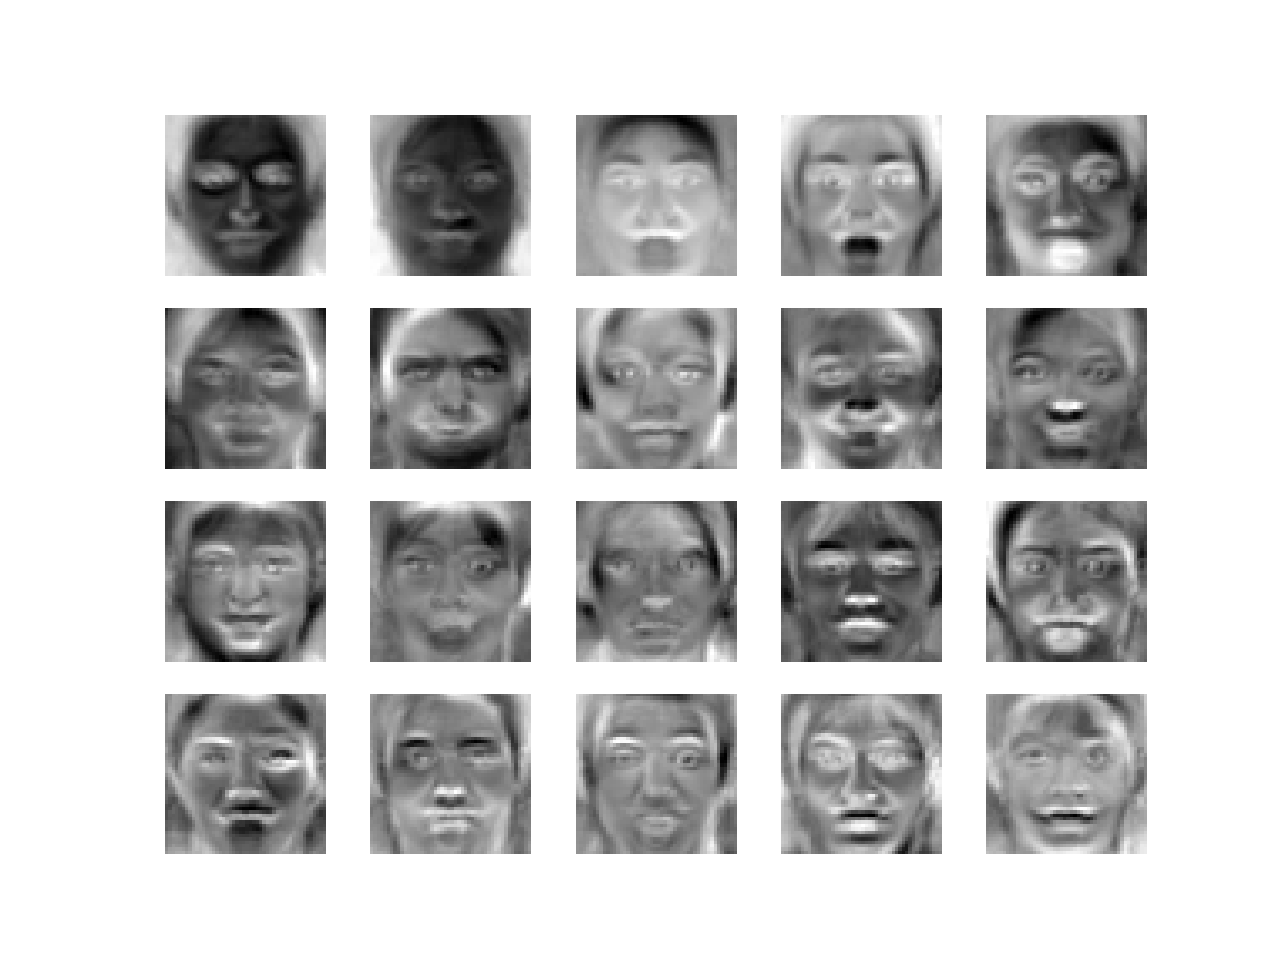
\includegraphics[width=0.9\linewidth]{Feature Extraction Images/eigenfaces.png}
   \caption{Eigenfaces for CK+48 Face Database.}
\end{center}
\begin{center}
    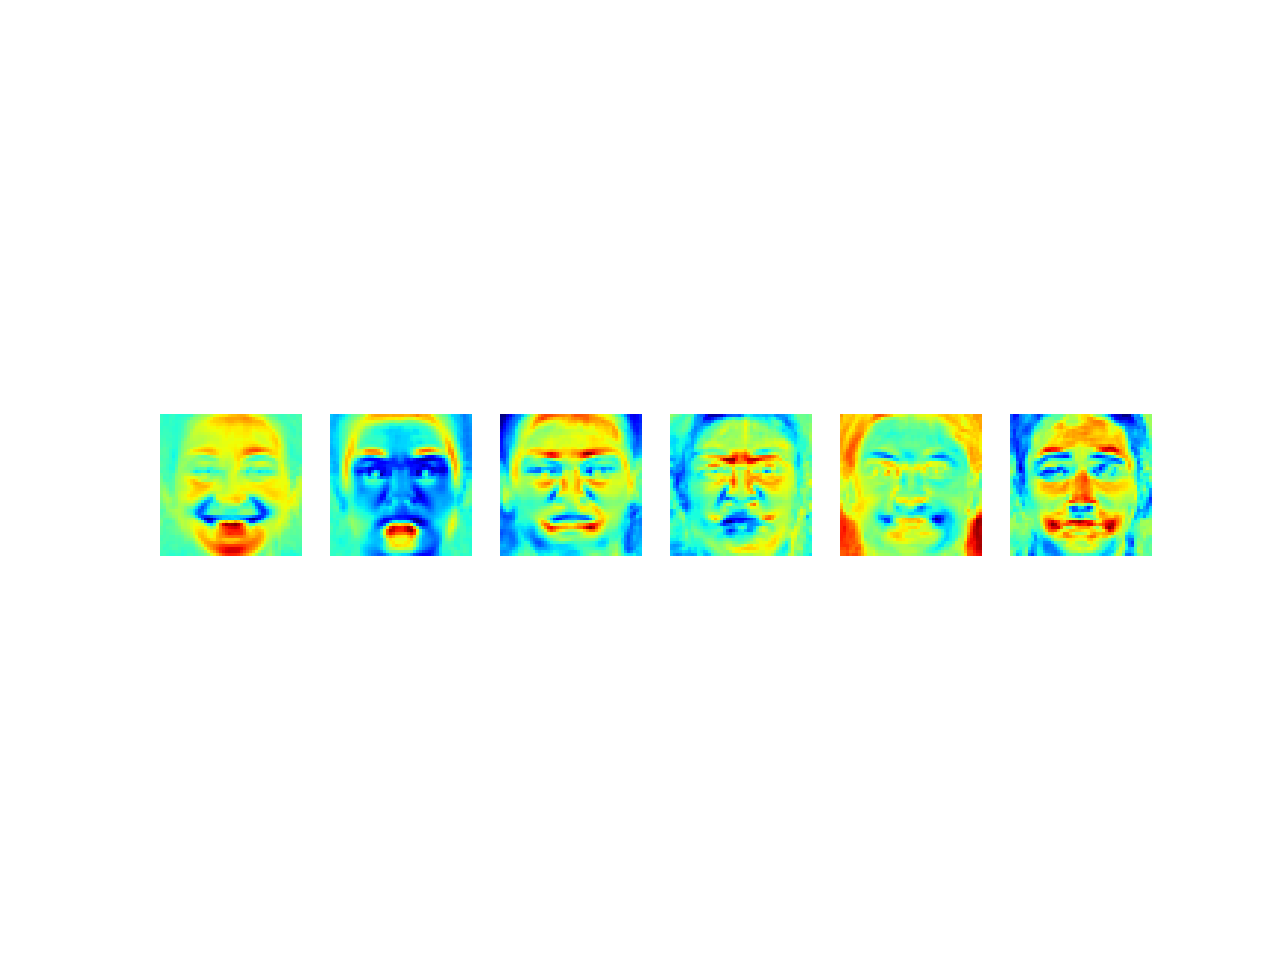
\includegraphics[width=0.9\linewidth]{Feature Extraction Images/fisherfaces.png}
   \caption{Fisherfaces (6 centroids) for 7 emotion labels of CK+48 Face Database.}
 \end{center}
\label{fig:long}
\label{fig:onecol}
\end{figure}

Fisherfaces takes the advantage of the fact the classes are actually linearly separable. It employs Fisher's Linear Discriminant (FLD), an class specific method that selects feature spaces in such a way that the ratio of the between-class scatter and the within-class scatter is maximized. Figure ~\ref{fig:fish-eigen-comparison} is a comparison of PCA and FLD for a two-class problem. One can see that while both PCA and FLD project the points from 2D down to 1D, PCA actually smears the classes together so that they are no longer linearly separable in the projected space, while FLD achieves greater between-class scatter, consequently simplifying the classification. \cite{Article06}

\begin{figure}[t]
\begin{center}
  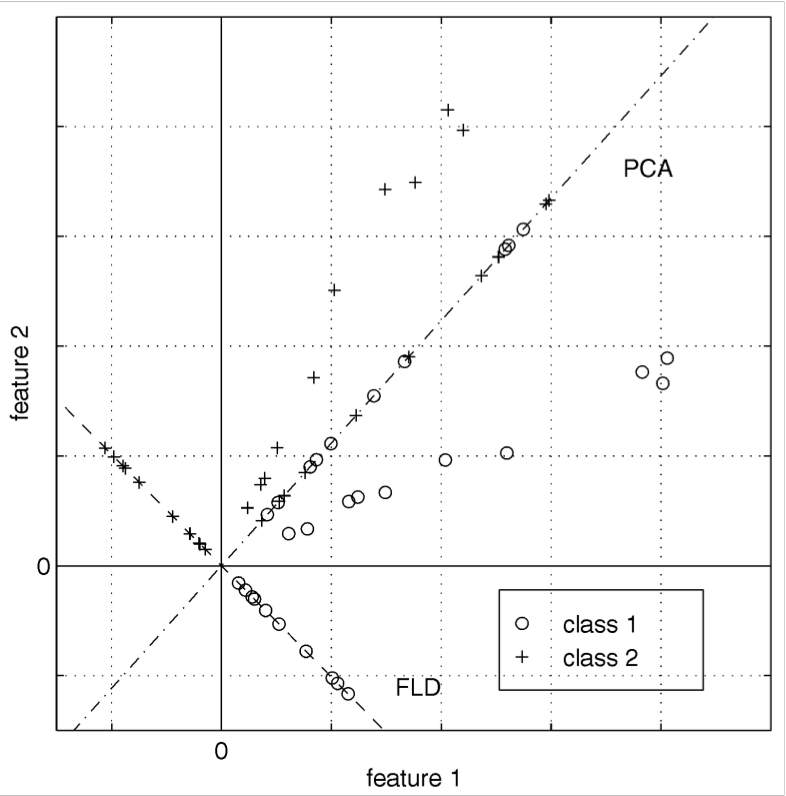
\includegraphics[width=0.8\linewidth]{fish-eigen-comparison.png}
  \caption{A comparison of principal component analysis (PCA) and Fisher’s linear discriminant (FLD) for a two class problem where data for each class lies near a linear subspace. \cite{Article06}}
  \label{fig:fish-eigen-comparison}
\end{center}
\end{figure}

In actual practice, however, using FLD alone in face detection may lead to problems. Formally, let us consider a set of $N$ sample images $\{\xvec_1, \xvec_2, \cdots, \xvec_N\}$ taking values in an $n$-dimension image space, and assume that each image belongs to one of $c$ classes $\{X_1, X_2, \cdots, X_c\}$. Now let the between-class scatter matrix be defined as
\[S_B = \sum\limits_{i = 1}^c N_i(\mu_i - \mu)(\mu_i - \mu)^T\]
and the within-class scatter matrix be defined as
\[S_W = \sum\limits_{i = 1}^c \sum\limits_{\xvec_k \in X_i} (\xvec_k - \mu_i)(\xvec_k - \mu_i)^T\]
where $\mu_i$ is the mean image of class $X_i$, and $N_i$ is the number of samples in class $X_i$. In FLD, we choose an optimal projection $W_{opt}$ such that it maximazes the ratio of the determinant of the between-class scatter matrix of the projected samples to the determinant of the within-class scatter matrix of the projected samples, i.e.
\begin{align*}
    W_{opt} &= \argmax_W \frac{|W^T S_B W|}{|W^T S_W W|} \\
    &= \begin{bmatrix}\wvec_1 & \wvec_2 & \cdots & \wvec_m\end{bmatrix}
\end{align*}
where $\{\wvec_i | i = 1, 2, \cdots, m\}$ is the set of generalized eigenvectors of $S_B$ and $S_W$ corresponding to the $m$ largest genrealized eigenvalues $\{\lambda_i | i = 1, 2, \cdots, m\}$. This will work when $S_W$ is non-singular. 

However, since the rank of $S_W$ is at most $N - c$ and the number of images in the learning set $N$ is much smaller than the number of pixels in each image $n$, one can observe that the within-class scatter matrix $S_W$ is always singular. This means that it is possible to choose the matrix $W$ such that the within-class scatter of the projected samples can be made exactly zero. 

To overcome this issue aroused by a singular $S_W$, the Fisherfaces combines FLD and PCA. In specific, it performs PCA to reduce the dimension of the feature space to $N - c$, and then applying the standard FLD to further reduce the dimension to $c - 1$. Formally, the optimal projection $W_{opt}$ in Fisherfaces algorithm is given by
\[W_{opt}^T = W_{fld}^T W_{pca}^T\]
where
\begin{align*}
    W_{pca} &= \argmax_W |W^T S_T W| \\
    W_{fld} &= \argmax_W \frac{|W^T W_{pca}^T S_B W_{pca} W|}{|W^T W_{pca}^T S_W W_{pca} W|}
\end{align*}
Here, 
\[S_T = \sum\limits_{i = 1}^N (\xvec_k - \mu_i)(\xvec_k - \mu_i)^T\]
where $n$ is the number of sample images, and $\mu \in \R^n$ is the mean image of all samples. Further experiments have indicated that Fisherfaces appears to outperform Eigenfaces in exterior variations including lighting, as well as simultaneously handling variation in lighting and expression. \cite{Article06}

In our system, we take the same methodology as Fisherfaces, but we rely on it to perform facial expression recognitions instead of face recognitions as it was originally suggested for.

\section{Our Approach}
The highly versatile facial expression recognition system we are suggesting works in the following approaches. When an image is fed to the system: 
\begin{enumerate}
    \item \textbf{Face Localization: }The Viola-Jones object detection framework is used to find a human face that appears in the image; For each face found, crop that area out and use Viola-Jones object detection framework again to find their eyes, then align the face by letting the line connecting two eyes turn to horizontal. At last, crop aligned faces out again, reshape them to 48 $\times$ 48 pixels and convert to gray-scale.
    \item \textbf{Feature Extraction: }After the face is detected, a converted Fisherfaces algorithm is employed to reduce the dimension of features demonstrated on the face; the algorithm incorporates PCA and FLD in the same manner as the original Fisherfaces does, but uses the model to process features for facial expressions instead of human faces.
    \item \textbf{Facial Expression Classfication: }After the features on the facial expression have been processed by the converted Fisherfaces algorithm, it is fed to a 1-Dimension Convolutional Neural Network Classifier for expression classification. The neural network was trained for 100 epochs using hyperparameters as shown in table ~\ref{tab:cnn_hp} below. 
    \begin{table}[h!]
        \centering
        \begin{tabular}{|c|c|c|} \hline
            Layer & Output Shape & \# of Parameters \\ \hline\hline
            Convolution 1D & $1 \times 32$ & 60032 \\ \hline
            Leaky ReLU & $1 \times 32$ & 0 \\ \hline
            Max Pooling 1D & $1 \times 32$ & 0 \\ \hline
            Dropout 25\% & $1 \times 32$ & 0 \\ \hline
            Convolution 1D & $1 \times 64$ & 6208 \\ \hline
            Leaky ReLU & $1 \times 64$ & 0 \\ \hline
            Max Pooling 1D & $1 \times 64$ & 0 \\ \hline
            Dropout 25\% & $1 \times 64$ & 0 \\ \hline
            Convolution 1D & $1 \times 128$ & 24704 \\ \hline
            Leaky ReLU & $1 \times 128$ & 0 \\ \hline
            Max Pooling 1D & $1 \times 128$ & 0 \\ \hline
            Dropout 40\% & $1 \times 128$ & 0 \\ \hline
            Flatten & 128 & 0 \\ \hline
            Dense & 128 & 16512 \\ \hline
            Leaky ReLU & 128 & 0 \\ \hline
            Dropout 30\% & 128 & 0 \\ \hline
            Dense & 7 & 903 \\ \hline
        \end{tabular}
        \caption{The Hyperparameters used to train the 1-Dimension Convolutional Neural Network Classifier.}
        \label{tab:cnn_hp}
    \end{table}
    
    Note that in each layer, a portion of the data are dropped out so as to reduce the reliance of the trained model to the training data set, in attempt to prevent overfitting. 

\end{enumerate}

\section{Experimental Results}
\subsection{Face Databases}

We evaluate the proposed method on well-known publicly available facial expression databases: CK+48 \cite{Article08}, and FER2013 \cite{Article10}. In this section we briefly review the content of these databases. 

\textbf{CK+48}: The Cohn-Kanade (CK) \cite{Article08} database was released for the purpose of promoting research into automatically detecting individual facial expressions. Since then, the CK database has become one of the most widely used test-beds for algorithm development and evaluation. The Cohn-Kanade (CK) \cite{Article08} database includes 593 video sequences recorded from 123 subjects ranging from 18 to 30 years old. Subjects displayed different expressions starting from the neutral for all sequences, and some sequences are labeled with basic expressions. \cite{Article09} And CK+48 is a cropped version of CK+, it extracted the last three frames from each sequence in the CK+ dataset \cite{Article08}, which contains a total of 981 facial expressions.

\textbf{FER2013}: The Facial Expression Recognition 2013 (FER-2013) database was introduced in the ICML 2013 Challenges in Representation Learning. \cite{Article10} The database was created using the Google image search API and faces have been automatically registered. Faces are labeled as any of the six basic expressions as well as the neutral. The resulting database contains 35,887 images most of them in wild settings. \cite{Article09}

% Please add the following required packages to your document preamble:
% \usepackage{multirow}
% \usepackage{longtable}
% Note: It may be necessary to compile the document several times to get a multi-page table to line up properly
\begin{longtable}{|c|l|c|c|}
\hline
Model                     & Database & \multicolumn{1}{l|}{Eigenfaces} & \multicolumn{1}{l|}{Fisherfaces} \\ \hline
\endhead
%
\multirow{2}{*}{CNN}      & CK+48    & 78\%                            & 99\%                             \\ \cline{2-4} 
                          & FER2013  & 32\%                            & 35\%                             \\ \hline
\multirow{2}{*}{SVM}      & CK+48    & 32\%                            & 99\%                             \\ \cline{2-4} 
                          & FER2013  & 58\%                            & 59\%                             \\ \hline
\multirow{2}{*}{Adaboost} & CK+48    & 70\%                            & 97\%                             \\ \cline{2-4} 
                          & FER2013  & 31\%                            & 34\%                             \\ \hline
\multirow{2}{*}{MLP}      & CK+48    & 85\%                            & 95\%                             \\ \cline{2-4} 
                          & FER2013  & 34\%                            & 35\%                             \\ \hline
\caption{Average accuracy for all models on CK+48 and FER2013 database}
\label{tab:my-table}
\end{longtable}

\subsection{Results}

For each database, we split it into three parts: training, validation and test sets with a ratio of 0.7:0.15:0.15. In the evaluation process, we use GridSearchCV to exhaustively search over and tune the hyperparameters of the models and calculate the confusion matrix, mean squared error and evaluate the accuracy for each different models. Table 2 reports the average accuracy when classifying the images into the seven basic expressions. According to the table 2, overall all of the models generate a fairly better result on CK+48 database compared with FER2013. Since in the FER2013 database, there are many tilted faces and also faces covered by the corresponding subject's hands, thus leading to unsatisfactory results. Figures ~\ref{fig:pca_projection}, ~\ref{fig:lda_projection} and ~\ref{fig:fer_pca_proj}, ~\ref{fig:fer_lda_proj} show the projection result onto the first 2 principal components and linear discriminants of eigenfaces and fisherfaces respectively on database CK+48 and FER2013. We can clearly see that the projection result for CK+48 is much better than that of FER2013, which accords the accuracy result in the table 2. In addition, fisherfaces performs better than eigenfaces on database CK+48 while on the FER2013, the eigenfaces and fisherfaces have the similar projection result according to Figure ~\ref{fig:fer_pca_proj} and ~\ref{fig:fer_lda_proj}. In summary, for CK+48 database all models perform better and achieve around 95\% with algorithm fisherfaces compared with eigenfaces. But on FER2013 database, except that SVM has a around 60\% average accuracy, the rest of models achieve around 31\% accuracy for both fisherfaces and eigenfaces.

Please be advised: Since we randomly shuffled our datasets into training, test and validation sets in data preprocessing step, these accuracies might be slightly different in each run.

\begin{figure}[t]
\begin{center}
  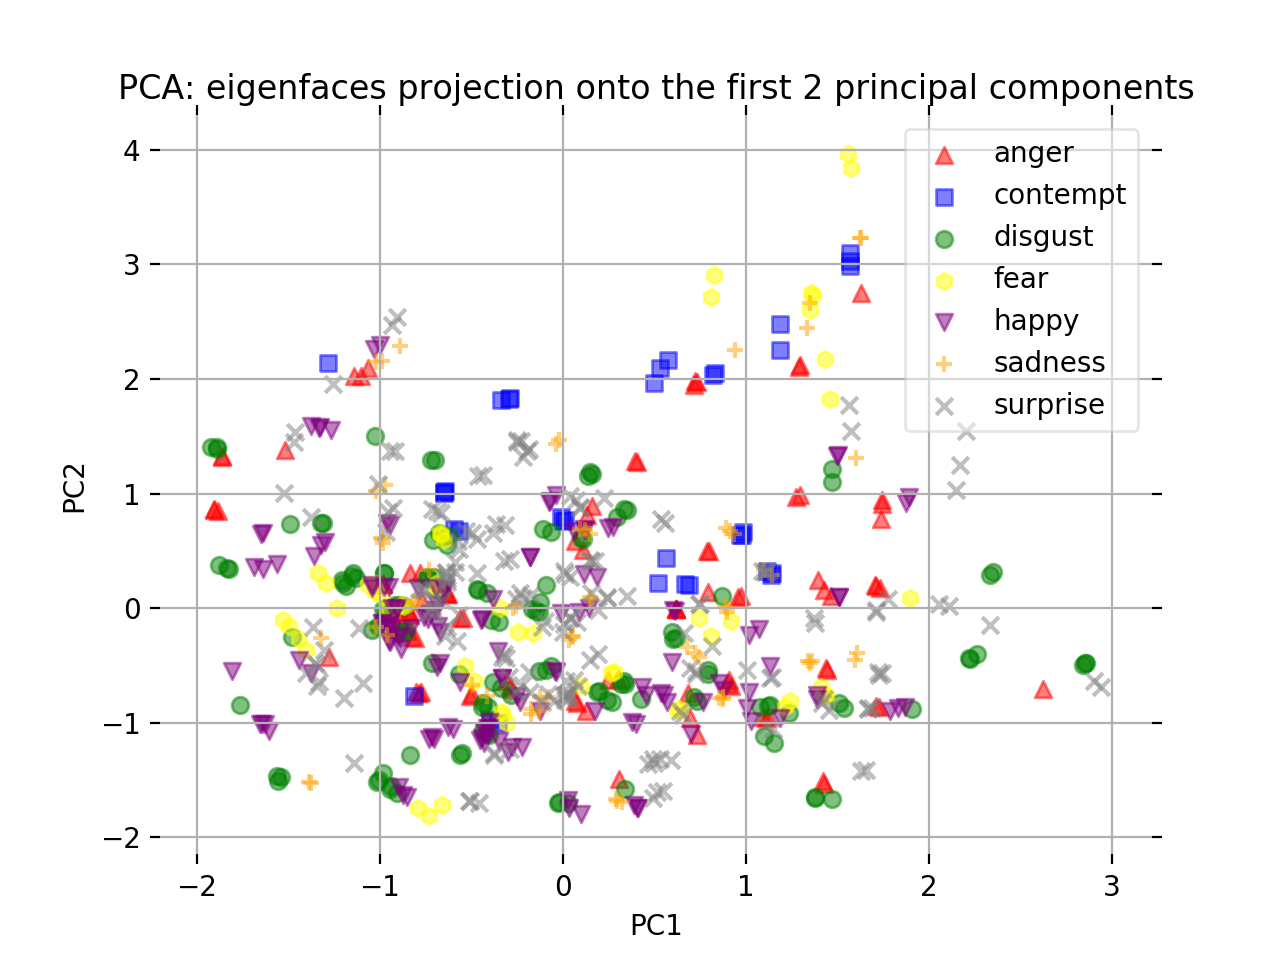
\includegraphics[width=0.8\linewidth]{Feature Extraction Images/pca_projection.png}
  \caption{PCA: eigenfaces of database CK+48 projection onto the first 2 principal components.}
  \label{fig:pca_projection}
\end{center}
\end{figure}

\begin{figure}[t]
\begin{center}
  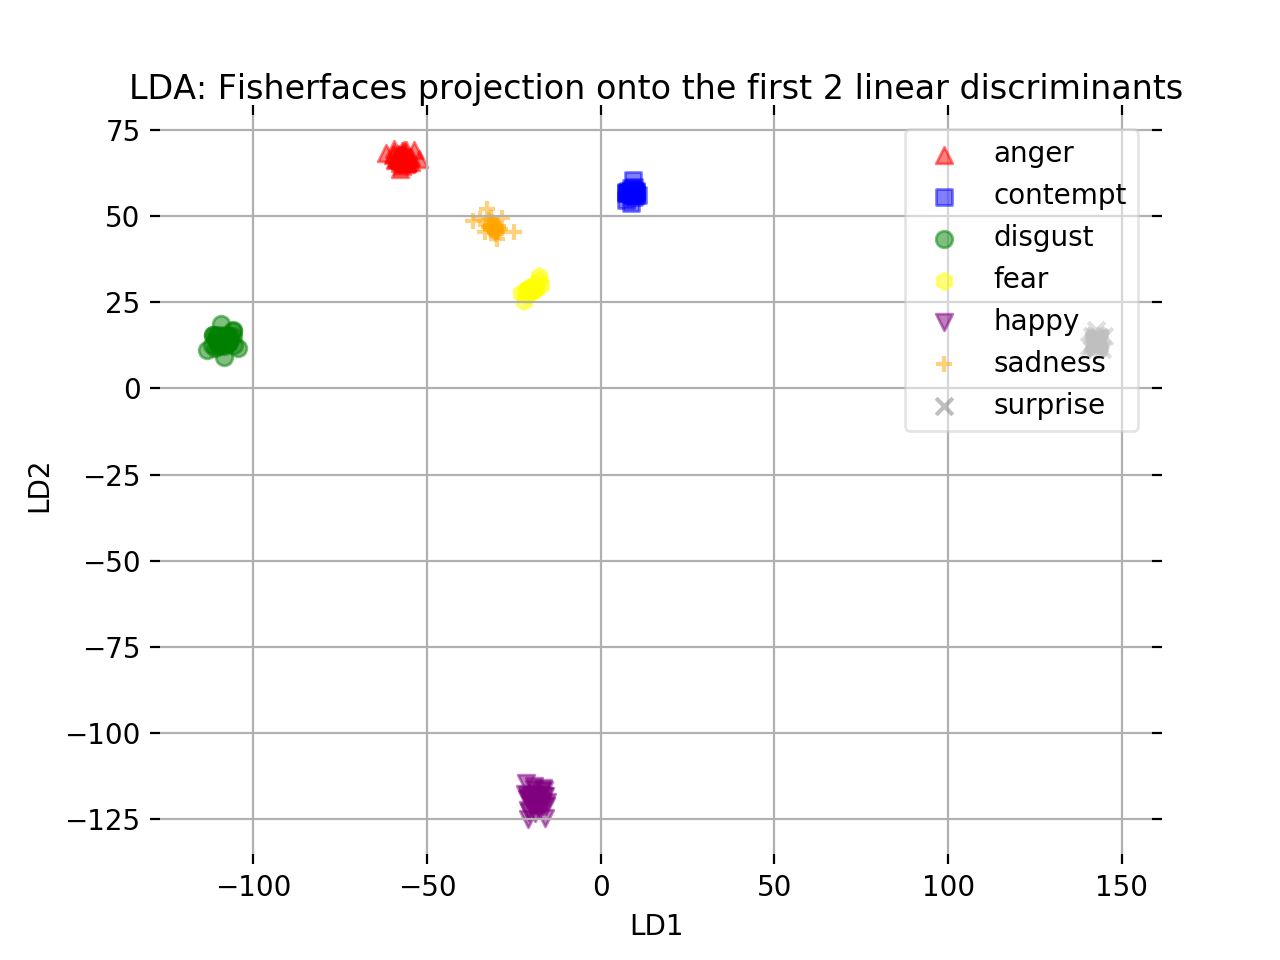
\includegraphics[width=0.8\linewidth]{Feature Extraction Images/lda_projection.png}
  \caption{LDA: fisherfaces of database CK+48 projection onto the first 2 linear discriminants.}
  \label{fig:lda_projection}
\end{center}
\end{figure}

\begin{figure}[t]
\begin{center}
  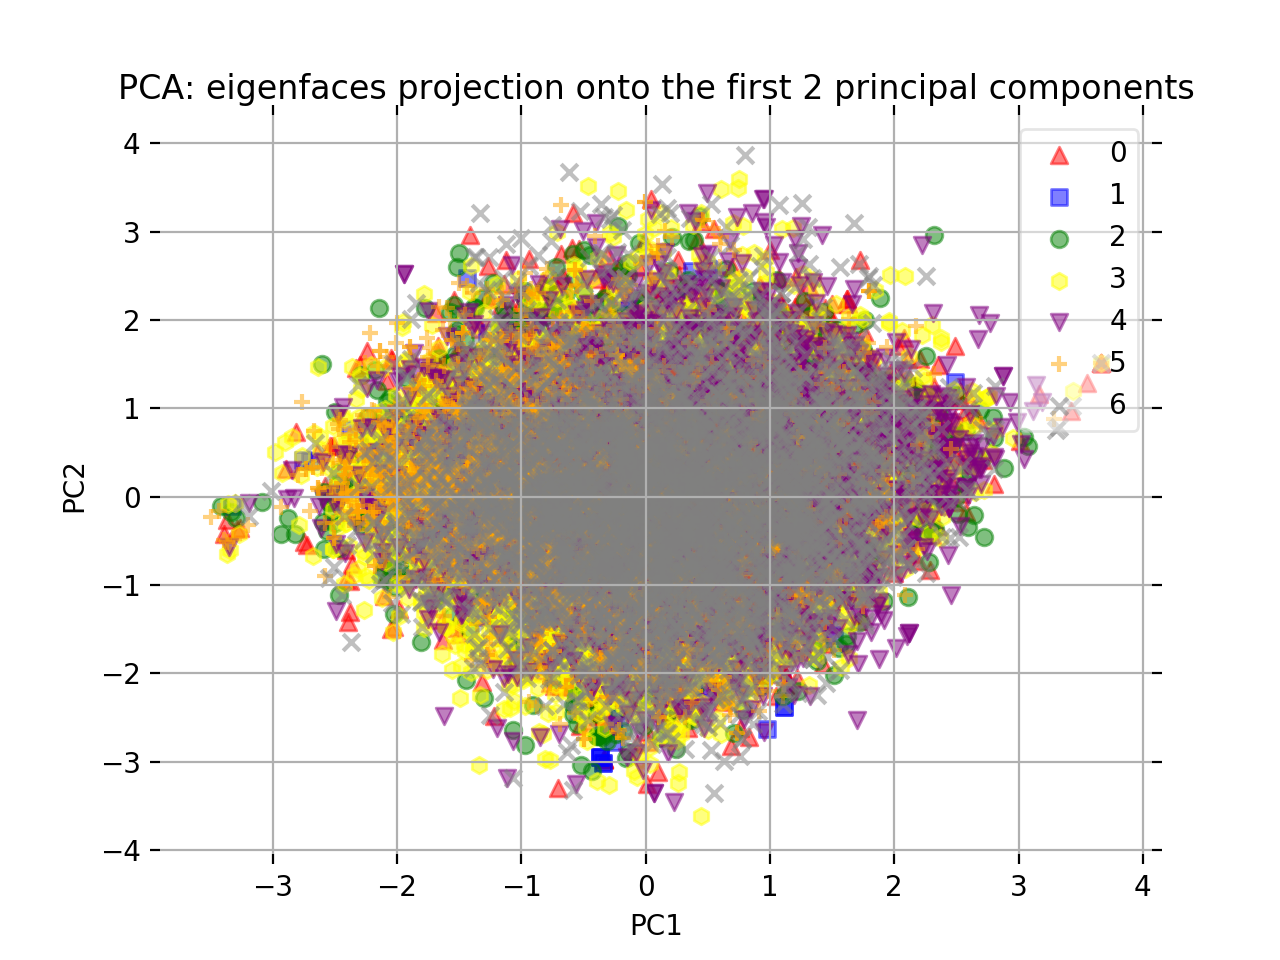
\includegraphics[width=0.8\linewidth]{Feature Extraction Images/fer2013_pca_projection.png}
  \caption{PCA: eigenfaces of database FER2013 projection onto the first 2 principal components. \cite{Article06}}
  \label{fig:fer_pca_proj}
\end{center}
\end{figure}

\begin{figure}[t]
\begin{center}
  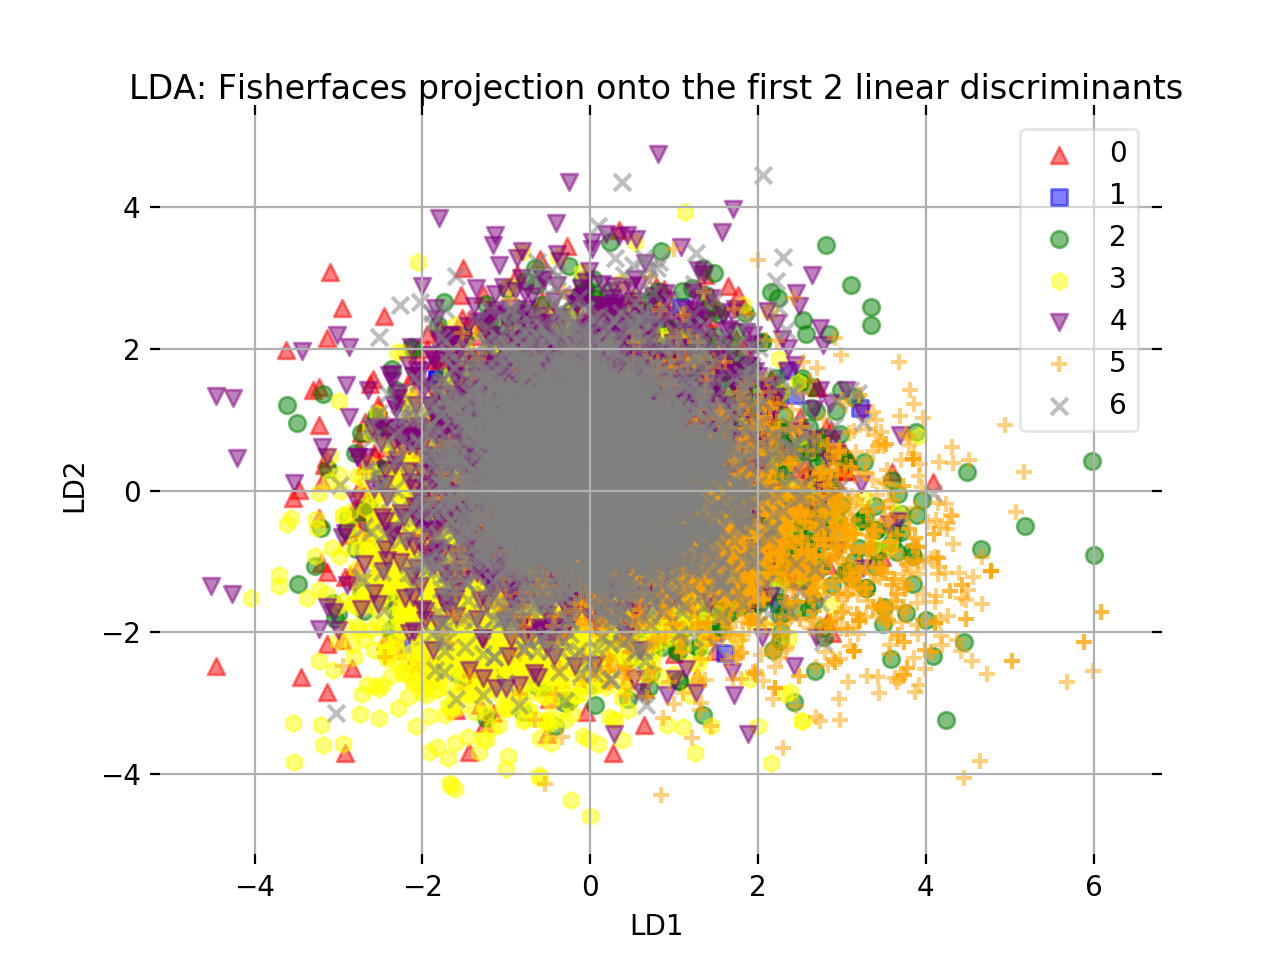
\includegraphics[width=0.8\linewidth]{Feature Extraction Images/fer2013_lda_projection.png}
  \caption{LDA: fisherfaces of database FER2013 projection onto the first 2 linear discriminants. \cite{Article06}}
  \label{fig:fer_lda_proj}
\end{center}
\end{figure}

\section{Conclusion and Future Work}

In this report, a highly versatile facial expression recognition system is proposed as a solution of face detection and emotion analysis. And we also combine the eigenfaces and fisherfaces algorithms with several different models to classify the images into some basic expressions and evaluate their accuracy respectively. Due to the computational constraints of training and evaluating, many techniques to improve performance was not employed in this project. In particular, some additional techniques including weighting the loss for class balancing, pre-training a more complex network with more layers using bigger filters such as ALexNet and VGGNet on a large database were left unexplored. In the future work, we would use a bigger and more varied database with equal race distributions to eliminate bias and pre-train other CNN's with more complex architecture. And we would also apply the method of weighting the loss for class balancing to improve the overall performance of the system.

\section{Authors’ Contributions}
\begin{itemize}
    \item Wei Cui: Refactoring all the codes, codes relate to data preprocess, feature extraction, model construction and evaluation using CNN, final report.
    \item Kewei Qiu: Codes relate to face detection and alignment, model construction and evaluation using SVM, AdaBoost and MLP, final report.
    \item Chenhao Gong: Codes relate to model construction and evaluation using CNN, presentation slides, README.md and final report.
\end{itemize}

{\small
\bibliographystyle{ieee_fullname}
\bibliography{mainbib}
}

\end{document}